%% ---------------------------------------------------------------------------
%% Safety-First Maternal Risk Screening
%% IEEE journal manuscript (IEEEtran, journal mode).
%%
%% Build:  latexmk -pdf main.tex
%%   or:   pdflatex main && bibtex main && pdflatex main && pdflatex main
%%
%% NOTE ON URDU. pdflatex cannot typeset Urdu script. The Urdu deliverable is
%% therefore presented through Fig. 5 (an interface capture) and through
%% romanised transliteration with English glosses in Table IX. Do not paste raw
%% Urdu glyphs into this source; switch the whole document to XeLaTeX with a
%% Nastaliq font first (see README.md in this directory).
%% ---------------------------------------------------------------------------
% Submission format. For a double-spaced single-column review copy, swap to:
%   \documentclass[journal,onecolumn,draftclsnofoot,12pt]{IEEEtran}
\documentclass[journal]{IEEEtran}

\usepackage{amsmath}
\usepackage{amssymb}
\usepackage{graphicx}
\usepackage{booktabs}
\usepackage{array}
\usepackage{multirow}
\usepackage{url}
\usepackage[hidelinks]{hyperref}

\graphicspath{{../../docs/img/}}

% Compact table typography; IEEE columns are narrow and these tables are wide.
\newcommand{\hdr}[1]{\textbf{#1}}
\newcommand{\best}[1]{\textbf{#1}}
\newcommand{\pmv}[2]{$#1 \pm #2$}

\begin{document}

\title{Safety-First Maternal Risk Screening: Documented\\ Clinical Thresholds as a Baseline, Label-Transfer\\ Calibration, and Urdu Risk Communication\\ as a Deliverable}

\author{Laiba~Mazhar%
% TODO(author): replace with your actual department, institution, city and
% country before submission. This is a placeholder, not a real affiliation.
\thanks{L. Mazhar is with \textsc{[Department]}, \textsc{[Institution]},
\textsc{[City]}, Pakistan (e-mail: laiba@cloudworksventures.com).}%
\thanks{\textbf{Provenance notice.} Every quantitative result reported in this
manuscript was computed on a deterministic \emph{synthetic} stand-in for the UCI
Maternal Health Risk dataset, not on the real file. The results demonstrate that
the pipeline, the metrics, and the analyses behave as specified; they are
\emph{not} findings about maternal health. Section~\ref{sec:synthetic} explains
the construction and the reasoning. Claims whose direction could plausibly
reverse on real data are flagged in place.}%
\thanks{\textbf{Not a medical device.} The described system is a research
prototype. It is not registered or certified with any regulatory authority, has
not been validated on any patient population, does not diagnose any condition,
and must not be used to make clinical decisions.}%
\thanks{Code, data card, and the full artefact set are available at
\url{https://github.com/laiba-mazhar/maternal-health-risk}.}}

\markboth{IEEE Journal of Biomedical and Health Informatics,~Vol.~XX, No.~X, August~2026}%
{Mazhar: Safety-First Maternal Risk Screening}

\maketitle

% ---------------------------------------------------------------------------
\begin{abstract}
Maternal risk classification on the UCI Maternal Health Risk dataset has
converged on a single research shape: preprocess, train a tree ensemble, report
accuracy in the low-to-mid eighties, and conclude that machine learning is
promising for maternal healthcare. We argue that this shape leaves three gaps
unaddressed. It optimises a metric that cannot distinguish the two error types
that matter clinically; it treats risk labels produced by an unpublished
protocol in one country as ground truth for deployment in another; and it stops
at a number, when the artefact a community health worker needs is a sentence she
can say to a family. We restructure the task around those gaps and contribute
(i)~a safety-first evaluation protocol built on a separately reported
\emph{critical-miss} rate, an asymmetric cost matrix, and referral thresholds
tuned under an operational budget nested inside the cross-validation loop;
(ii)~a label-transfer calibration study encoding eleven sourced obstetric
criteria as a transparent rule baseline; and (iii)~hand-authored Urdu risk
communication whose safety properties are enforced by continuous-integration
lint rules rather than reviewer diligence. Our headline result is negative and,
we argue, the most useful finding available here: no learned model beat the
eleven documented thresholds on high-risk recall, even after equalising referral
load ($0.918$ versus $0.847$ for the best learned model). The learned models
earn their place differently, cutting the catastrophic high-to-low error from
$3.5\%$ to $1.2\%$ or below and improving balanced accuracy from $0.642$ to
$0.700$, which supports a hybrid rules-plus-model design that the
accuracy-reporting framing never puts on the table. We further find that the
sampling condition of the dataset's \emph{undocumented} blood-glucose column
moves the clinical baseline more than any modelling choice available to us:
reading it as fasting rather than post-load glucose shifts guideline--label
agreement from $64.0\%$ to $31.4\%$.
\end{abstract}

\begin{IEEEkeywords}
Clinical decision support, cost-sensitive learning, explainable artificial
intelligence, external validity, health informatics, low-resource languages,
maternal health, model calibration.
\end{IEEEkeywords}

% ---------------------------------------------------------------------------
\section{Introduction}
\IEEEPARstart{P}{akistan's} maternal mortality ratio remains among the higher
figures in South Asia~\cite{pmms2019}, and the majority of maternal deaths
worldwide are caused by conditions detectable in advance: hypertensive
disorders, haemorrhage, sepsis, and complications of pre-existing
disease~\cite{say2014global}. In much of rural Pakistan the first clinical
contact is not an obstetrician but a Lady Health Worker
(LHW)~\cite{lhw-evaluation,bhutta2011community}, who can take a blood pressure,
a temperature, a pulse, and a glucose strip, and who must then make a single
decision: refer, or not.

That decision is the intervention. Anything a screening tool does that does not
improve it --- including its accuracy figure --- is decoration. This framing
drives every choice in this paper and is where we depart from existing work.

\subsection{Three Properties of a Useful Screening Tool}

\subsubsection{It must weight errors the way the clinic does}
Roughly $37\%$ of this cohort is labelled low risk, so a classifier predicting
``low risk'' for every mother attains $37\%$ accuracy while missing $100\%$ of
high-risk cases. This is not a straw man: it is the direction any unweighted
loss pushes a model on imbalanced data. Worse, accuracy treats \emph{predicting
mid risk for a high-risk mother} --- which still escalates her --- as identical
to \emph{predicting low risk}, which sends her home. Those errors differ in
kind, not degree.

\subsubsection{It must not assume its labels transfer}
The dataset was collected through a community health-monitoring initiative in
Bangladesh~\cite{ahmed-iot-maternal}, and its labelling protocol was never
published: we do not know which guideline, if any, the labellers applied, nor
how disagreements were resolved. Treating those labels as ground truth for a
Pakistani deployment embeds an untested transfer assumption at the root of the
model --- the failure mode systematic reviews of clinical prediction models find
repeatedly~\cite{wynants2020covid,vancalster2019calibration}.

\subsubsection{Its output must be deliverable at the point of care}
A probability, or a risk band in clinical English, is not something an LHW can
say to a family in rural Punjab. The last mile --- a sentence that is
understood, believed, and acted upon --- is where a screening programme succeeds
or fails~\cite{kelly2019challenges}, and it is almost entirely absent from the
machine-learning literature on this dataset.

\subsection{Contributions}
\begin{enumerate}
\item A \textbf{safety-first evaluation protocol} (Section~\ref{sec:metrics})
whose primary quantities are high-risk recall, a separately tracked
critical-miss rate, expected cost under an asymmetric matrix, and referral load;
in which the decision rule is separated from the classifier and tuned under an
explicit referral budget \emph{inside} the cross-validation loop; and in which
model selection is on recall rather than accuracy.
\item A \textbf{label-transfer calibration study}
(Section~\ref{sec:calibration-results}) encoding eleven sourced obstetric
criteria as a transparent rule baseline, measuring agreement, directionality of
disagreement, and per-criterion discriminative contribution.
\item A \textbf{matched-referral comparison} (Section~\ref{sec:matched}) that
equalises operational cost before comparing a threshold-tuned model against a
fixed clinical rule --- the only form of that comparison we consider honest.
\item \textbf{Urdu risk communication as a first-class, testable deliverable}
(Section~\ref{sec:communication}), hand-authored rather than machine-translated,
with three safety commitments enforced as executable lint rules.
\item A \textbf{reproducible artefact} in which every reported number is
regenerated by a single command and stamped with its data provenance.
\item A \textbf{negative headline result} (Section~\ref{sec:matched}) and an
analysis of what the learned models do buy, which points to a hybrid design.
\end{enumerate}

% ---------------------------------------------------------------------------
\section{Related Work}

\subsection{Machine Learning on the UCI Maternal Health Dataset}
Since the dataset's release~\cite{uci-maternal-health,ahmed-iot-maternal}, a
substantial body of work has applied the standard tabular toolkit to it:
decision trees, random forests, gradient boosting, occasionally a small neural
network, usually with SMOTE~\cite{chawla2002smote} or class weighting for the
imbalance, typically reporting accuracy and macro F1 in the low-to-mid eighties.
We are not aware of prior work on this dataset that reports a class-specific
safety metric, separates the decision threshold from the classifier, or compares
against a guideline-derived rule baseline.

\subsection{Obstetric Risk Scoring}
Clinical obstetric risk scoring predates machine learning and is built from
documented thresholds rather than fitted parameters. That literature supplies
the criteria we encode in Section~\ref{sec:baseline}; what it does not supply is
an account of what a learned model adds over it, which is the question
Section~\ref{sec:matched} asks directly.

\subsection{Evaluation Methodology for Clinical Prediction Models}
The methodological literature has been explicit for years that discrimination
alone is insufficient, that calibration is where deployed models
fail~\cite{vancalster2019calibration,steyerberg2014abcd}, and that the
decision-analytic question --- what does acting on this model cost and gain ---
requires net-benefit reasoning rather than a threshold-free
summary~\cite{vickers2006dca}. Our referral-budget constraint and
matched-referral comparison are a coarse, discrete instance of that reasoning:
rather than integrating net benefit across thresholds, we fix the operational
cost and compare recall there. TRIPOD~\cite{tripod2015} asks for the provenance
and transfer analysis that Section~\ref{sec:calibration-results} provides.
Cost-sensitive learning provides the formal basis for the asymmetric matrix we
adopt~\cite{elkan2001cost}.

\subsection{Explainability in Clinical Machine Learning}
We use SHAP~\cite{lundberg2017shap} in its exact forms: TreeSHAP for the
ensembles~\cite{lundberg2020trees} and the closed-form linear explainer for the
logistic model. Our contribution here is epistemic rather than methodological:
we require the attribution method to be named in every output, so a silent
fallback to an approximate method cannot be presented as SHAP. Rudin's argument
for interpretable models in high-stakes settings~\cite{rudin2019stop} is
relevant to our outcome, since the model selected on safety grounds turned out
to be the interpretable one.

\subsection{Health Communication and Low-Resource Languages}
Work on health communication establishes that comprehension, trust, and
actionability determine whether advice is followed. The machine-learning
literature on this dataset does not engage with it. Machine translation of
clinical instructions is not a safe substitute, as a mistranslated instruction
is a safety incident rather than a quality defect.

\subsection{Data Documentation and Proxy Labels}
Datasheets~\cite{gebru2021datasheets} presume that provenance is recoverable.
Where it is not --- as with the glucose sampling condition here --- the
practical recipe is to state the assumption and measure what it costs, which is
what Section~\ref{sec:calibration-results} does. Obermeyer
\emph{et~al.}~\cite{obermeyer2019bias} showed how a proxy label can encode a
systematic inequity that accuracy cannot see; the analogue here is milder but
structurally identical.

% ---------------------------------------------------------------------------
\section{Gap Analysis and Positioning}

Table~\ref{tab:gaps} consolidates the gaps left by prior work and maps each to
the section addressing it. Our aim is explicitly \emph{not} to improve on
published accuracy figures --- Section~\ref{sec:cv-results} shows our models land
in the same band. It is to argue that the figure was never the interesting
quantity.

\begin{table}[!t]
\renewcommand{\arraystretch}{1.25}
\caption{Gaps in Existing Work and Where This Paper Addresses Them}
\label{tab:gaps}
\centering
\footnotesize
\begin{tabular}{@{}p{0.05\columnwidth}p{0.55\columnwidth}p{0.24\columnwidth}@{}}
\toprule
\hdr{ID} & \hdr{Gap left by existing work} & \hdr{Addressed in} \\
\midrule
G1 & Symmetric metrics cannot express that high$\rightarrow$low is
categorically worse than high$\rightarrow$mid &
Sec.~\ref{sec:metrics}, \ref{sec:cv-results} \\
G2 & Dataset labels assumed to transfer; provenance and units treated as
settled & Sec.~\ref{sec:baseline}, \ref{sec:calibration-results} \\
G3 & No clinical floor; no account of what learning adds over documented rules
& Sec.~\ref{sec:baseline}, \ref{sec:matched} \\
G4 & Thresholds implicit (\texttt{argmax}) or tuned with leakage; referral load
an accident & Sec.~\ref{sec:decision}, \ref{sec:protocol} \\
G5 & ``We applied SHAP'' conceals method substitution and silent degenerate
output & Sec.~\ref{sec:attribution}, \ref{sec:attr-results} \\
G6 & Localisation absent or machine-translated; message quality treated as a
review activity & Sec.~\ref{sec:communication}, \ref{sec:msg-results} \\
G7 & Documentation frameworks presume recoverable provenance &
Sec.~\ref{sec:data-real}, \ref{sec:calibration-results} \\
\bottomrule
\end{tabular}
\end{table}

% ---------------------------------------------------------------------------
\section{Data}

\subsection{The Real Dataset, and One Load-Bearing Ambiguity}
\label{sec:data-real}

The UCI Maternal Health Risk Data Set contains approximately $1{,}014$ records
with six features --- age, systolic and diastolic blood pressure, blood glucose,
body temperature, and resting heart rate --- and an ordinal label in
$\{\text{low}, \text{mid}, \text{high}\}$ risk, distributed roughly
$406/336/272$. The imbalance runs in the worst direction: the class we least
want to miss is the smallest.

Three properties shape everything downstream.

\subsubsection{Units are undocumented, and one is load-bearing}
Body temperature is Fahrenheit (reading it as Celsius would be catastrophic) and
glucose is mmol/L, but the \emph{sampling condition} of the glucose column is
unrecorded. WHO thresholds for hyperglycaemia in pregnancy differ sharply by
sampling condition~\cite{who-hip-2013}, as shown in Table~\ref{tab:who}.

\begin{table}[!t]
\renewcommand{\arraystretch}{1.25}
\caption{WHO Thresholds for Hyperglycaemia in Pregnancy}
\label{tab:who}
\centering
\footnotesize
\begin{tabular}{@{}lcc@{}}
\toprule
\hdr{Reading} & \hdr{Gestational diabetes} & \hdr{Diabetes in pregnancy} \\
\midrule
Fasting plasma glucose & $5.1$--$6.9$ mmol/L & $\geq 7.0$ mmol/L \\
2-hour 75\,g OGTT      & $8.5$--$11.0$ mmol/L & $\geq 11.1$ mmol/L \\
\bottomrule
\end{tabular}
\end{table}

The observed range is roughly $6$--$19$ mmol/L with a median near $8$. Read as
fasting values, over $80\%$ of a community \emph{screening} cohort would be
diabetic, which is not credible; read as post-load values the distribution is
clinically ordinary. We therefore assume the OGTT reading, state the assumption
explicitly, and report the sensitivity of every guideline result to it
(Section~\ref{sec:calibration-results}) --- following the spirit
of~\cite{gebru2021datasheets} for the case where documentation is already
unrecoverable.

\subsubsection{Some values are physiologically impossible}
Heart rates of $7$ bpm are dropped digits, not bradycardic patients; ages up to
$70$ are not maternal ages. We repair these by class-conditional median
imputation rather than dropping the row, preserving the five other usable vitals
on an affected record.

\subsubsection{Two clinical criteria cannot fire}
Diastolic pressure never reaches the severe-hypertension threshold of $110$
mmHg, and heart rate never exceeds $90$ bpm, so the tachycardia criterion
($>100$) is unreachable. We retain both and report them as \emph{silent}: a
criterion whose cut-off the data cannot reach is a fact about the data, and
dropping it would conceal that fact.

\subsection{The Synthetic Stand-In, and the Status of Every Number Here}
\label{sec:synthetic}

All numbers in this manuscript were computed on a deterministic synthetic
dataset generated to resemble published summaries of the real file. This was a
project constraint rather than a methodological choice, and we state it plainly:
\textbf{nothing in Section~\ref{sec:results} is a finding about maternal
health.} The results demonstrate that the pipeline runs, that the metrics behave
as designed, and that the analyses produce the shape of answer they claim to.

The generator samples a class from the published class proportions, then samples
vitals from class-conditional normal distributions clipped to the published
per-column ranges and discretised as a clinic form would record them. It
deliberately injects the real file's awkward properties --- implausible heart
rates, exact duplicate rows, and $7\%$ label noise concentrated on the mid/high
boundary --- because a stand-in cleaner than the real data would let the
pipeline pass tests it would fail in practice. Class-conditional centres were
chosen so that guideline thresholds \emph{partially} agree with the labels:
perfect agreement would render the calibration study vacuous, and total
disagreement would mean measuring the generator rather than anything real.

Synthetic provenance propagates into every artefact --- the metadata record,
every generated table, the interface banner, and the figures, where the stamp is
burned into the image rather than left in the caption, because a figure pasted
into a slide deck loses its caption long before it loses its axes. An automated
test asserts this propagation.

% ---------------------------------------------------------------------------
\section{Method}

\subsection{Guideline Criteria as a First-Class Baseline}
\label{sec:baseline}

We encode eleven obstetric criteria drawn from published guidance, each stored
as data with its threshold, severity, and source, so that a clinician can review
the rule set without reading code:

\begin{itemize}
\item \textbf{Hypertension}~\cite{isshp2018}: systolic $140$--$159$ or diastolic
$90$--$109$ mmHg (moderate); systolic $\geq 160$ or diastolic $\geq 110$
(severe).
\item \textbf{Hyperglycaemia in pregnancy}~\cite{who-hip-2013}: $8.5$--$11.0$
mmol/L (moderate); $\geq 11.1$ (severe), under the OGTT reading of
Section~\ref{sec:data-real}.
\item \textbf{Fever}~\cite{who-imppc}: $100.4$--$101.9^\circ$F, i.e.\
$\geq 38^\circ$C (moderate); $\geq 102^\circ$F (severe).
\item \textbf{Tachycardia}: resting heart rate $>100$ bpm (moderate).
\item \textbf{Maternal age}~\cite{who-anc-2016}: $<18$ or $\geq 35$ years
(moderate).
\end{itemize}

These combine through an escalation rule chosen to be defensible rather than
clever: any severe feature yields high risk; two or more moderate features yield
high risk; exactly one yields mid risk; none yields low risk.

This baseline serves two purposes. As a comparator it sets the floor a learned
model must clear to justify its complexity. As an instrument it lets us ask
whether the dataset's labels agree with published guidance at all
(Section~\ref{sec:calibration-results}).

\subsection{Safety-First Metrics}
\label{sec:metrics}

Let the ordinal classes be indexed $0$ (low), $1$ (mid), $2$ (high). We report,
in this order:

\begin{itemize}
\item \textbf{High-risk recall}: the fraction of high-risk mothers escalated at
all.
\item \textbf{Critical-miss rate}: the fraction of high-risk mothers predicted
\emph{low} risk,
\begin{equation}
\mathrm{CMR} = \frac{|\{i : y_i = 2 \wedge \hat{y}_i = 0\}|}{|\{i : y_i = 2\}|}.
\end{equation}
Reported separately from recall because ``mid risk'' still escalates her while
``low risk'' does not --- the difference between a delayed referral and no
referral.
\item \textbf{Expected cost}: mean cost under an asymmetric matrix $C$ with
$C_{2,0}=25$, $C_{2,1}=8$, $C_{1,0}=4$, and over-escalation priced at $1$--$2$.
The values encode a clinical judgement, not a measurement; they are isolated in
configuration so they can be challenged.
\item \textbf{Referral rate}: the share of mothers escalated above low risk.
This is the operational cost, and it is a first-class metric because the quiet
way a screening tool fails is by referring so many mothers that the programme
stops believing it.
\item Conventional metrics --- accuracy, balanced accuracy, macro F1, and
quadratic-weighted $\kappa$~\cite{cohen1968weighted} --- reported for
comparability with published work, not for selection.
\end{itemize}

\subsection{A Decision Rule Separate from the Model}
\label{sec:decision}

Fitting a classifier and deciding where to place the referral threshold are
different acts, and conflating them is how safety-critical thresholds end up at
whatever \texttt{argmax} happened to produce. Given predicted class
probabilities $p = (p_0, p_1, p_2)$ and thresholds $(t_{\mathrm{high}},
t_{\mathrm{esc}})$, we assign
\begin{equation}
\hat{y} =
\begin{cases}
2 & \text{if } p_2 \geq t_{\mathrm{high}},\\
1 & \text{else if } p_1 + p_2 \geq t_{\mathrm{esc}},\\
0 & \text{otherwise.}
\end{cases}
\end{equation}
A $40\%$ chance of high risk therefore escalates even when low risk holds a
$45\%$ plurality --- a decision \texttt{argmax} cannot express.

Thresholds maximise high-risk recall \emph{subject to a referral budget}
($55\%$), ties broken on expected cost. The constraint is part of the objective
rather than a footnote: without it the optimum is always ``refer everybody'',
which has perfect recall and is switched off within a month.

\subsection{Protocol, Leakage Control, and the Matched Comparison}
\label{sec:protocol}

We use repeated stratified cross-validation, $5$ folds $\times$ $4$ repeats.
Because the referral thresholds are \emph{fitted parameters}, tuning them on the
rows used to score the model would leak. Each outer fold therefore tunes its
operating point on inner $3$-fold cross-validated probabilities computed from
that fold's training portion only, then applies the frozen point to the held-out
fold.

The model zoo comprises a majority-class baseline, the guideline baseline,
logistic regression, random forest, XGBoost~\cite{chen2016xgboost}, and a small
multilayer perceptron, all built on scikit-learn~\cite{scikit-learn}, with class
balancing throughout. Selection is on mean high-risk recall, tie-broken on
expected cost, with baselines excluded from selection but reported alongside.

The guideline rule has no threshold to tune; it refers whoever it refers.
Comparing it against a threshold-tuned model at each system's own operating
point is therefore not a comparison --- whichever refers more people wins on
recall by construction. We consequently push every learned model to the
guideline baseline's exact referral load and compare there.

\subsection{Attribution That Names Itself}
\label{sec:attribution}

Attributions come from exact SHAP where an exact explainer exists --- TreeSHAP
for the ensembles, the closed-form linear explainer for logistic regression ---
and degrade to permutation importance or occlusion otherwise. The method is
named in every output and every figure caption. An attribution silently swapped
beneath a plot labelled ``SHAP'' is worse than no plot.

Two implementation traps are worth recording. First, SHAP~0.49 cannot parse the
vector-valued \texttt{base\_score} that XGBoost~$\geq 3.0$ writes for
multi-class models; we route through XGBoost's own \texttt{pred\_contribs},
which computes the same exact values. Second, a linear SHAP explainer
constructed with the explained row as its own background returns
\emph{all-zero} attributions --- silently, with no error --- because every
feature equals its own background mean. Both are covered by regression tests.

\subsection{Communication as Part of the System}
\label{sec:communication}

Model output becomes a bilingual message through hand-authored templates. Urdu
is written by hand, not machine-translated, because a mistranslated clinical
instruction is a safety incident and because register matters as much as
vocabulary. Three commitments are enforced by lint rules executed in continuous
integration, so a well-meaning later edit fails the build rather than shipping:

\begin{enumerate}
\item \textbf{No catastrophising.} Urgency lives in the recommended action and
its timeframe (``today'', ``within a few days''), never in frightening
adjectives. A family that panics may go nowhere, or to the wrong place.
\item \textbf{No diagnosis.} The tool reports observations and names who to see.
It never names a condition, because it cannot confirm one.
\item \textbf{Family-inclusive framing at the high band.} Where care decisions
are made collectively, a message addressed only to the patient can stall against
a household that was never consulted.
\end{enumerate}

A fourth rule emerged from reviewing rendered output rather than from design:
\textbf{the low-risk band mentions no drivers at all.} Telling a mother her
result is normal and then listing which of her vitals ``stood out'' plants worry
the result does not justify, and worry is what makes a family ignore the next
message.

% ---------------------------------------------------------------------------
\section{Results}
\label{sec:results}

All results below are computed on the synthetic stand-in
(Section~\ref{sec:synthetic}).

\subsection{Cross-Validated Performance}
\label{sec:cv-results}

Table~\ref{tab:cv} reports the model zoo under the metric set of
Section~\ref{sec:metrics}. Three observations follow.

\begin{table*}[!t]
\renewcommand{\arraystretch}{1.3}
\caption{Cross-Validated Performance, 5 Folds $\times$ 4 Repeats (Mean $\pm$ Std).
Arrows Indicate the Direction of Improvement. Bold Marks the Best Value per Column.}
\label{tab:cv}
\centering
\begin{tabular}{@{}lcccccc@{}}
\toprule
\hdr{Model} & \hdr{High-risk recall $\uparrow$} & \hdr{Critical miss $\downarrow$}
& \hdr{Expected cost $\downarrow$} & \hdr{Referral rate $\downarrow$}
& \hdr{Balanced acc. $\uparrow$} & \hdr{Accuracy $\uparrow$} \\
\midrule
Guideline baseline   & \best{\pmv{0.900}{0.041}} & \pmv{0.036}{0.027} & \best{\pmv{1.010}{0.221}} & \pmv{0.633}{0.019} & \pmv{0.656}{0.031} & \pmv{0.640}{0.033} \\
Logistic regression  & \pmv{0.730}{0.059} & \pmv{0.044}{0.029} & \pmv{1.290}{0.201} & \pmv{0.542}{0.019} & \best{\pmv{0.759}{0.020}} & \best{\pmv{0.764}{0.018}} \\
Multilayer perceptron& \pmv{0.716}{0.054} & \pmv{0.036}{0.022} & \pmv{1.269}{0.161} & \pmv{0.548}{0.025} & \pmv{0.758}{0.020} & \pmv{0.764}{0.019} \\
XGBoost              & \pmv{0.663}{0.065} & \pmv{0.034}{0.024} & \pmv{1.395}{0.227} & \best{\pmv{0.535}{0.023}} & \pmv{0.740}{0.027} & \pmv{0.750}{0.025} \\
Random forest        & \pmv{0.648}{0.047} & \best{\pmv{0.029}{0.019}} & \pmv{1.383}{0.186} & \pmv{0.542}{0.024} & \pmv{0.744}{0.022} & \pmv{0.755}{0.021} \\
Majority baseline    & $0.000$ & $1.000$ & \pmv{8.417}{0.034} & $0.000$ & $0.333$ & \pmv{0.370}{0.001} \\
\bottomrule
\end{tabular}
\end{table*}

First, the majority baseline attains $37\%$ accuracy --- respectable-looking ---
while missing every high-risk mother, at roughly six times the expected cost of
the worst real model. This is the concrete form of the argument in
Section~\ref{sec:metrics}: a metric on which the degenerate model appears merely
mediocre rather than disqualified is not a safety metric.

Second, our learned models land in the accuracy band the literature reports
($0.750$ to $0.764$), so this is not a story about a weak implementation. They
are simply being asked a different question.

Third, selection on recall changes the answer. Logistic regression is selected
--- the simplest and most inspectable of the learned models. Note that random
forest achieves the \emph{lowest} critical-miss rate ($0.029$) while having the
worst high-risk recall ($0.648$): it rarely commits the catastrophic error but
under-escalates into the mid band more often. Reporting only one of those two
numbers would misrepresent it in either direction.

\subsection{Do the Dataset's Labels Agree with Published Guidance?}
\label{sec:calibration-results}

Exact agreement between guideline bands and dataset labels is $64.0\%$, with
linear $\kappa = 0.584$ and quadratic-weighted $\kappa = 0.696$ --- substantial
ordinal agreement, but far from the interchangeability that treating these
labels as clinical ground truth would assume. Table~\ref{tab:confusion} and
Fig.~\ref{fig:calibration} give the joint distribution.

\begin{table}[!t]
\renewcommand{\arraystretch}{1.3}
\caption{Dataset Labels Versus Guideline Bands}
\label{tab:confusion}
\centering
\footnotesize
\begin{tabular}{@{}lccc@{}}
\toprule
& \multicolumn{3}{c}{\hdr{Guideline band}} \\
\cmidrule(l){2-4}
\hdr{Dataset label} & low & mid & high \\
\midrule
low $(370)$  & $267$ & $88$  & $15$ \\
mid $(350)$  & $90$  & $121$ & $\mathbf{139}$ \\
high $(281)$ & $10$  & $18$  & $253$ \\
\bottomrule
\end{tabular}
\end{table}

\begin{figure}[!t]
\centering
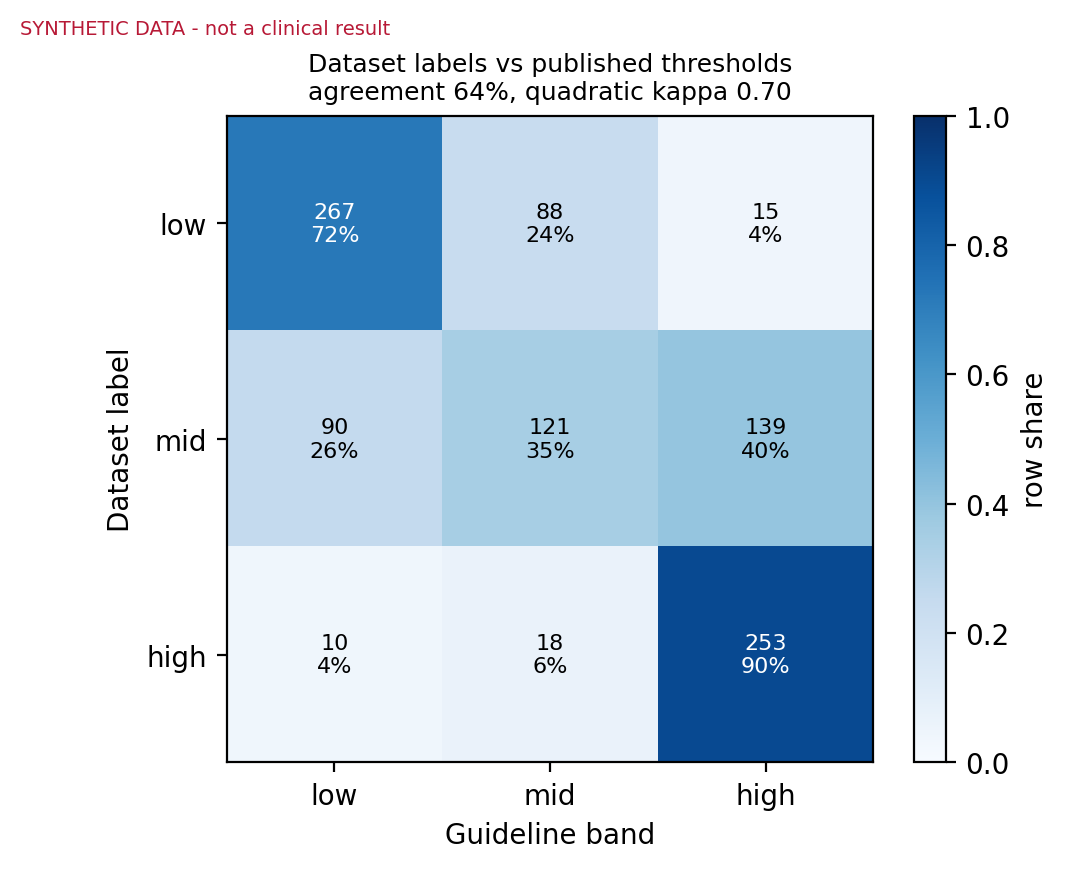
\includegraphics[width=0.92\columnwidth]{fig3_guideline_calibration.png}
\caption{Dataset labels against guideline bands, normalised by row. Exact
agreement $64.0\%$, quadratic-weighted $\kappa = 0.696$. Computed on synthetic
data.}
\label{fig:calibration}
\end{figure}

The disagreement has structure rather than being symmetric noise.

\subsubsection{The guidelines are stricter in the middle}
Of $350$ mothers the dataset labels mid risk, $139$ ($40\%$) reach the guideline
\emph{high} band. Whatever protocol the labellers used was more permissive than
published thresholds on precisely the ambiguous cases.

\subsubsection{Ten percent of dataset high-risk mothers fall below the guideline
high band}
Published thresholds alone would not escalate $28$ of $281$ --- a direct
argument against replacing a learned model with a rule sheet.

\subsubsection{A third of the rule set does almost all the work}
Table~\ref{tab:activity} and Fig.~\ref{fig:activity} report per-criterion firing
rates. The diabetes-in-pregnancy criterion fires for $69.4\%$ of high-risk
mothers and $0\%$ of low-risk ones; advanced maternal age for $51.2\%$ versus
$4.1\%$. Two criteria never fire at all, for the reason given in
Section~\ref{sec:data-real}.

\begin{table}[!t]
\renewcommand{\arraystretch}{1.2}
\caption{Guideline Criterion Firing Rates (\%) by Dataset Label}
\label{tab:activity}
\centering
\footnotesize
\begin{tabular}{@{}lccccc@{}}
\toprule
\hdr{Criterion} & \hdr{Sev.} & \hdr{All} & \hdr{low} & \hdr{mid} & \hdr{high} \\
\midrule
Diabetes in pregnancy      & S & $25.1$ & $0.0$  & $16.0$ & $69.4$ \\
Advanced maternal age      & M & $25.1$ & $4.1$  & $26.3$ & $51.2$ \\
Gest.\ hypertension (dia.) & M & $15.5$ & $2.2$  & $9.7$  & $40.2$ \\
Gestational diabetes       & M & $21.1$ & $6.5$  & $36.3$ & $21.4$ \\
Gest.\ hypertension (sys.) & M & $10.4$ & $0.0$  & $8.9$  & $26.0$ \\
Adolescent pregnancy       & M & $11.6$ & $14.3$ & $12.3$ & $7.1$  \\
Fever                      & M & $4.9$  & $1.9$  & $4.3$  & $9.6$  \\
High fever                 & S & $3.0$  & $1.9$  & $1.7$  & $6.0$  \\
Severe systolic hypert.    & S & $1.0$  & $0.0$  & $0.0$  & $3.6$  \\
Severe diastolic hypert.   & S & $0.0$  & $0.0$  & $0.0$  & $0.0$  \\
Tachycardia                & M & $0.0$  & $0.0$  & $0.0$  & $0.0$  \\
\bottomrule
\end{tabular}
\\[2pt]
\raggedright\footnotesize S: severe; M: moderate. The final two criteria are
\emph{silent}: the recorded ranges cannot reach their cut-offs.
\end{table}

\begin{figure}[!t]
\centering
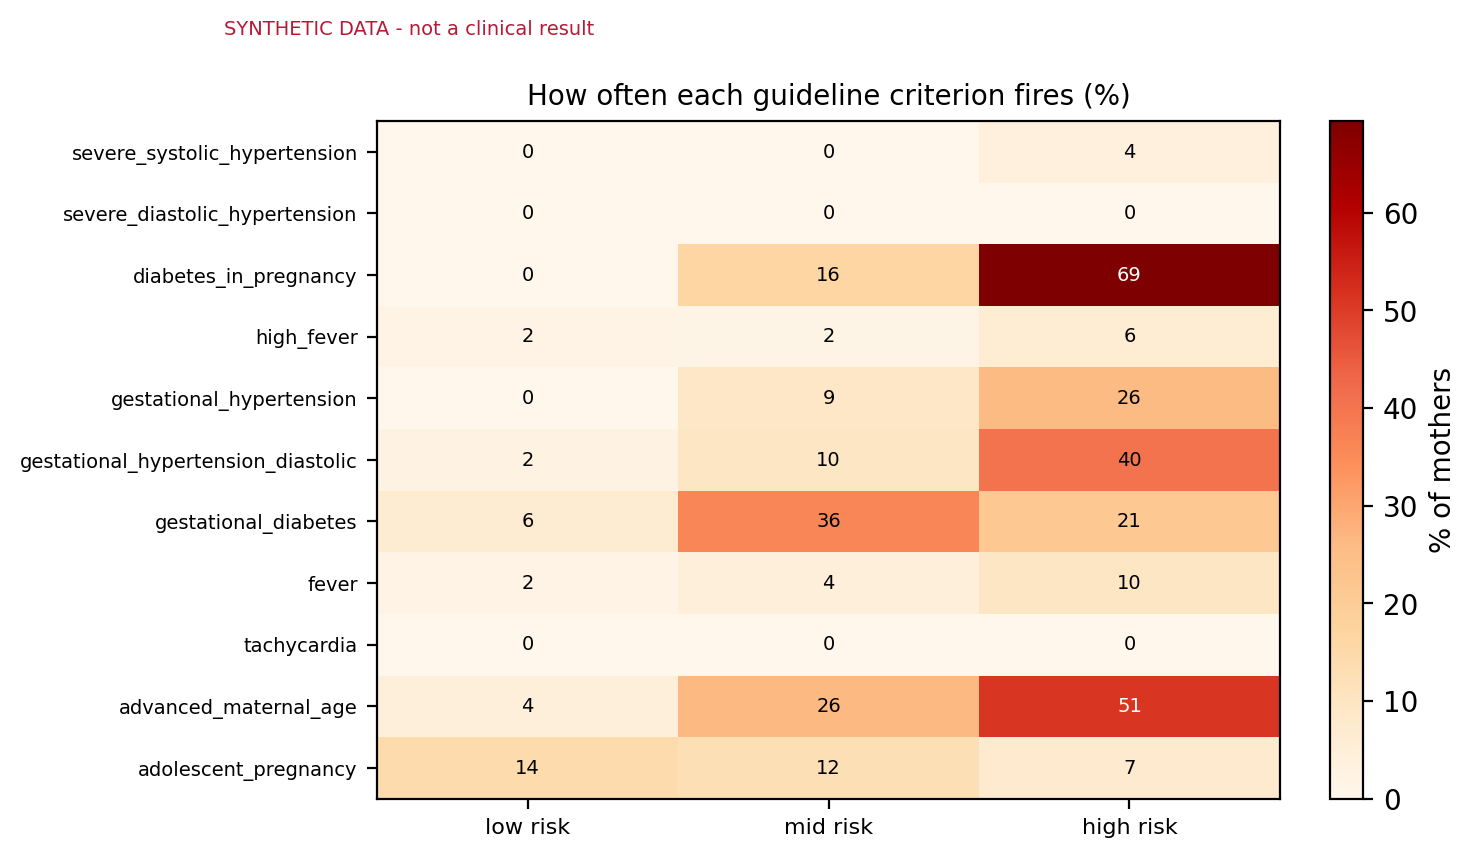
\includegraphics[width=0.98\columnwidth]{fig4_rule_activity.png}
\caption{Per-criterion firing rates by dataset label. Two criteria are
unreachable given the recorded ranges and are retained as silent rather than
dropped.}
\label{fig:activity}
\end{figure}

\subsubsection{One undocumented column dominates}
Table~\ref{tab:bs} reports the sensitivity of the guideline baseline to the
glucose interpretation. Switching from post-load to fasting moves agreement from
$64.0\%$ to $31.4\%$, quadratic $\kappa$ from $0.696$ to $0.136$, and the share
of mothers escalated from $40.7\%$ to $82.0\%$.

\begin{table}[!t]
\renewcommand{\arraystretch}{1.3}
\caption{Sensitivity to the Undocumented Glucose Sampling Condition}
\label{tab:bs}
\centering
\footnotesize
\begin{tabular}{@{}lcccc@{}}
\toprule
\hdr{Interpretation} & \hdr{Cut-offs} & \hdr{Agreement} & \hdr{$\kappa_q$} & \hdr{Flagged high} \\
\midrule
2-hour OGTT (assumed) & $8.5 / 11.1$ & $0.640$ & $0.696$ & $40.7\%$ \\
Fasting               & $5.1 / 7.0$  & $0.314$ & $0.136$ & $82.0\%$ \\
\bottomrule
\end{tabular}
\end{table}

This is our clearest methodological finding: the sampling condition of a single
undocumented column changes the clinical baseline more than any model
architecture, hyperparameter, or threshold in the study. Work that trains on
this dataset without stating its glucose interpretation has left the most
consequential assumption in the analysis unstated.

\subsection{Does Learning Beat the Guidelines at Equal Cost?}
\label{sec:matched}

Table~\ref{tab:matched} forces every learned model to the guideline baseline's
referral load ($\approx 0.648$). Fig.~\ref{fig:tradeoff} shows the full
trade-off.

\begin{table*}[!t]
\renewcommand{\arraystretch}{1.3}
\caption{Performance at the Guideline Baseline's Referral Load}
\label{tab:matched}
\centering
\begin{tabular}{@{}lccccc@{}}
\toprule
\hdr{Model} & \hdr{Referral rate} & \hdr{High-risk recall $\uparrow$}
& \hdr{Critical miss $\downarrow$} & \hdr{Expected cost $\downarrow$}
& \hdr{Balanced acc. $\uparrow$} \\
\midrule
Guideline baseline    & $0.648$ & \best{$0.918$} & $0.035$ & $0.993$ & $0.642$ \\
Logistic regression   & $0.648$ & $0.847$ & $0.012$ & \best{$0.907$} & $0.700$ \\
Multilayer perceptron & $0.638$ & $0.835$ & $0.012$ & $0.887$ & \best{$0.731$} \\
XGBoost               & $0.648$ & $0.788$ & \best{$0.000$} & $0.930$ & $0.715$ \\
Random forest         & $0.651$ & $0.776$ & \best{$0.000$} & $0.987$ & $0.699$ \\
\bottomrule
\end{tabular}
\end{table*}

\begin{figure}[!t]
\centering
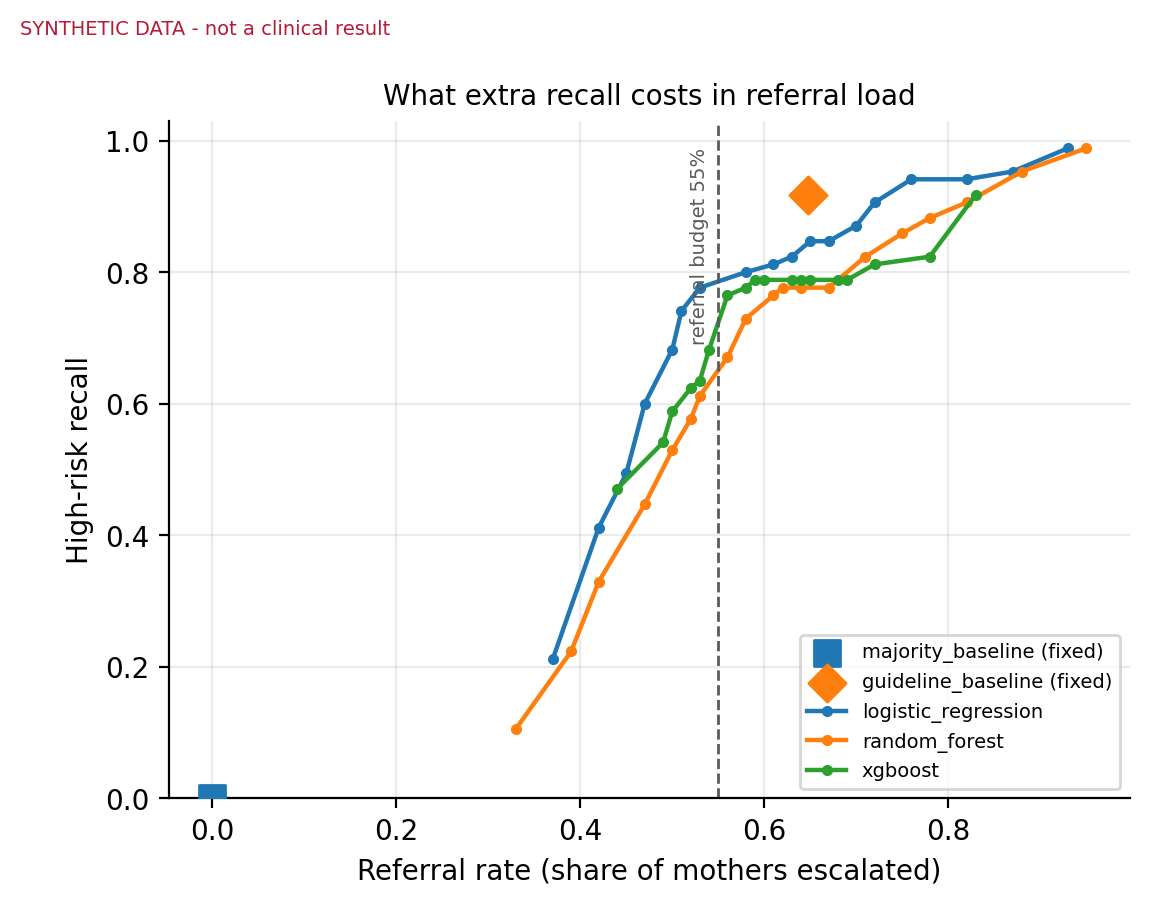
\includegraphics[width=0.98\columnwidth]{fig5_recall_vs_referral.png}
\caption{High-risk recall against referral load. The guideline baseline (marker)
sits above every learned model's achievable curve at its own referral rate. The
dashed line is the $55\%$ referral budget. Computed on synthetic data.}
\label{fig:tradeoff}
\end{figure}

\textbf{No learned model beats eleven documented thresholds on high-risk recall,
even at matched referral load.} The gap is not marginal: $0.918$ against $0.847$
for the best learned model. We report this as the headline because it is the
result a reader most needs and the one this literature's framing tends to
obscure. On the project's own primary metric, the machine learning did not win.

What the learned models buy is a different error profile. The rule baseline
sends $3.5\%$ of high-risk mothers home as low risk; logistic regression sends
$1.2\%$, and both tree ensembles send none. The guideline rule catches more
high-risk mothers overall yet is \emph{more} likely to place one in the worst
possible band, because a fixed rule has no graded confidence to fall back on:
when no criterion fires, it says low risk with no hedge available. Expected cost
is correspondingly lower for logistic regression ($0.907$) and the MLP ($0.887$)
than for the rule baseline ($0.993$), and balanced accuracy is substantially
better ($0.700$--$0.731$ versus $0.642$).

The defensible claim is therefore narrower and more interesting than ``our model
is better'': at equal operational cost, the learned models trade a little
high-risk recall for near-elimination of the worst individual error and a better
overall cost profile. A deployment would sensibly use both --- the rules as a
non-overridable safety net, the model to grade everything the rules leave
silent. \emph{This is the claim most at risk of reversing on real data.}

\subsection{Attribution}
\label{sec:attr-results}

Exact LinearSHAP on the selected model ranks blood glucose first by a wide
margin, then systolic and diastolic pressure, age, heart rate, and body
temperature (Table~\ref{tab:shap}, Fig.~\ref{fig:importance}). TreeSHAP on the
random forest and on XGBoost produces the same ordering. Agreement across three
model families and two exact SHAP implementations is a validity signal: glucose
and blood pressure dominating a maternal-risk model is clinically expected, and
a model leaning on body temperature would have been suspect regardless of its
accuracy. The ordering also matches the rule-activity analysis of
Section~\ref{sec:calibration-results} --- two methods, one built from published
thresholds and one from fitted coefficients, agreeing on which vitals carry the
signal.

\begin{table}[!t]
\renewcommand{\arraystretch}{1.3}
\caption{Feature Attribution, Exact LinearSHAP on the Selected Model}
\label{tab:shap}
\centering
\footnotesize
\begin{tabular}{@{}lcccc@{}}
\toprule
\hdr{Vital} & \hdr{Mean $|$SHAP$|$} & \hdr{low} & \hdr{mid} & \hdr{high} \\
\midrule
Blood glucose    & $\mathbf{1.091}$ & $1.637$ & $0.233$ & $1.405$ \\
Systolic BP      & $0.525$ & $0.788$ & $0.152$ & $0.636$ \\
Diastolic BP     & $0.446$ & $0.626$ & $0.044$ & $0.669$ \\
Age              & $0.252$ & $0.379$ & $0.089$ & $0.289$ \\
Heart rate       & $0.190$ & $0.285$ & $0.080$ & $0.205$ \\
Body temperature & $0.120$ & $0.138$ & $0.042$ & $0.181$ \\
\bottomrule
\end{tabular}
\end{table}

\begin{figure}[!t]
\centering
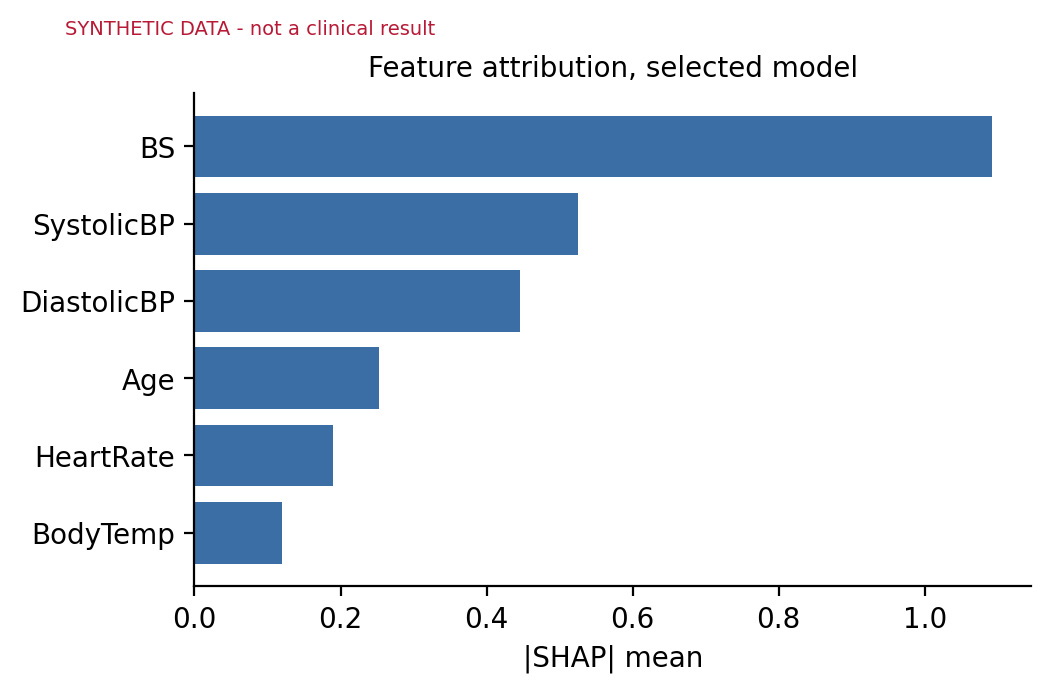
\includegraphics[width=0.92\columnwidth]{fig6_feature_importance.png}
\caption{Feature attribution for the selected model. Method named in the
artefact rather than assumed.}
\label{fig:importance}
\end{figure}

\subsection{Threshold Stability}
Tuned $t_{\mathrm{high}}$ values vary across folds, as expected at
$\sim 1{,}000$ rows with roughly $440$ rows per inner tuning set. We report the
spread rather than an averaged point estimate: a threshold that swings across
folds is not one to deploy, and a single mean would hide that.

\subsection{Message Safety}
\label{sec:msg-results}

All three band templates pass the lint gate in both languages. The suite
includes adversarial tests that inject a catastrophising phrase, a diagnosis
claim, and an action-free message, and assert the linter catches each --- the
linter is verified to have teeth rather than assumed to. Review status is
\texttt{UNREVIEWED} for all three bands, and a test asserts the artefact does
not claim otherwise. Fig.~\ref{fig:ui} shows the rendered high-risk output.

\begin{figure}[!t]
\centering
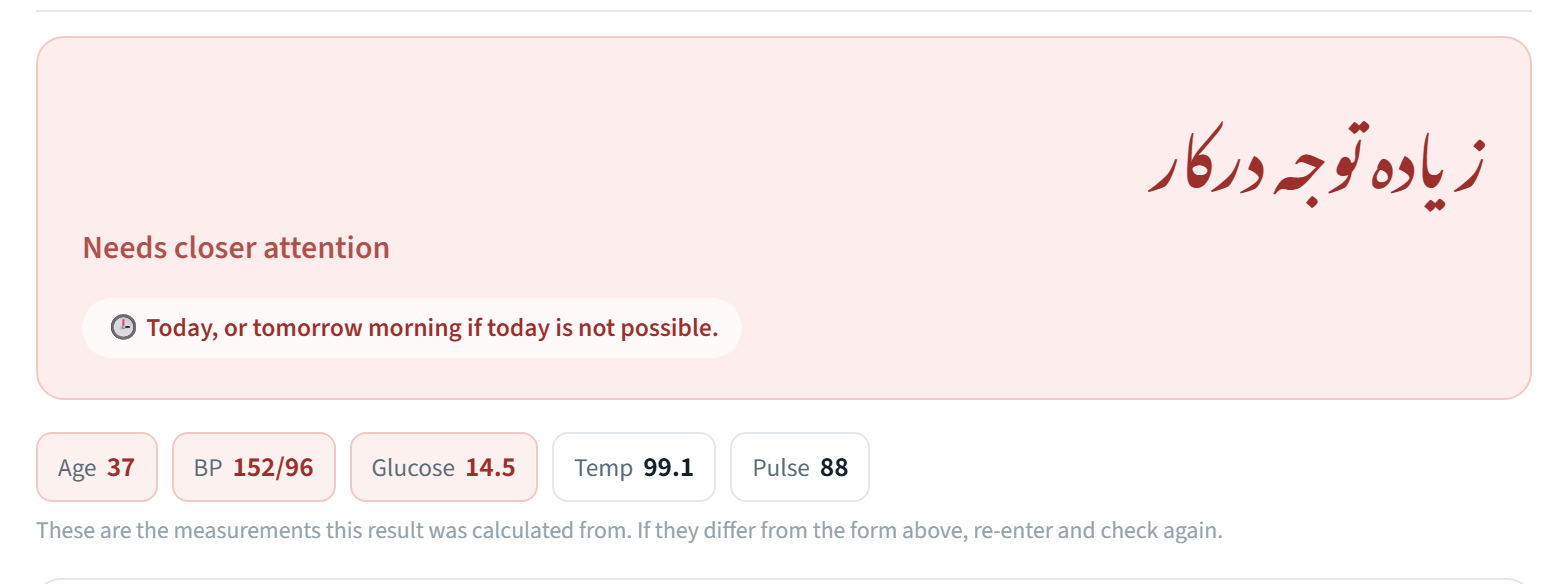
\includegraphics[width=0.98\columnwidth]{band-high.png}
\caption{Rendered high-risk output. The Urdu band name is set in Nastaliq and
precedes the English gloss; the timeframe carries the urgency; the measurement
chips restate exactly what was scored, with values crossing a guideline
threshold highlighted. Interface capture; synthetic data.}
\label{fig:ui}
\end{figure}

% ---------------------------------------------------------------------------
\section{Discussion}

\textbf{The negative result is the useful one.} A study designed to show that a
model beats a rule sheet, and which found the opposite, is more informative than
one reporting $84\%$ accuracy and stopping. It also carries a direct design
consequence: run the documented criteria as a non-overridable safety net and use
the model to grade the cases where no criterion fires. That hybrid is invisible
to the accuracy-reporting framing, because that framing never puts the rule
baseline on the table.

\textbf{Undocumented units are a bigger risk than model choice.}
Section~\ref{sec:calibration-results} found the glucose sampling condition moves
the clinical baseline far more than anything we varied in modelling. The lesson
is unglamorous: for small clinical tabular datasets, effort spent resolving
provenance with whoever collected the data will usually beat effort spent on
architecture. This extends the datasheet literature~\cite{gebru2021datasheets}
with a concrete recipe for the case where documentation is already unrecoverable
--- state the assumption, then measure what it costs.

\textbf{Label transfer is measurable, and cheap to measure.} Quadratic $\kappa$
of $0.696$ between dataset labels and published thresholds is substantial
agreement with a structured residue: the guidelines are systematically stricter
on ambiguous mid cases, so a model trained on these labels inherits the
labellers' permissiveness. This is an afternoon's work and it is what TRIPOD
asks for~\cite{tripod2015}.

\textbf{Interpretability was not a sacrifice.} Logistic regression was selected
on the project's own safety criterion, not chosen for simplicity. On six tabular
vitals that is the outcome~\cite{rudin2019stop} predicts, and it means the
deployed model has exactly computable attributions and reviewable coefficients
rather than a post-hoc story about a black box.

\textbf{Communication is not downstream polish.} The one design rule we did not
anticipate --- suppressing driver phrases at the low band --- came from reading
rendered Urdu, not from the model. It is invisible to every metric in
Section~\ref{sec:results} and would plausibly matter more to real-world outcomes
than the difference between our best and worst classifier. Encoding message
constraints as CI lint rather than as review guidelines is the component of this
work we would most readily reuse elsewhere.

% ---------------------------------------------------------------------------
\section{Threats to Validity}

\textbf{Construct validity.} The cost matrix is a judgement, not a measurement.
Pricing a critical miss at $25\times$ an unnecessary referral is defensible but
arbitrary, and expected-cost comparisons move with it. It is isolated in
configuration so it can be challenged; a sensitivity sweep is the obvious next
step.

\textbf{Internal validity.} Threshold tuning is nested to prevent leakage, but
with $\sim 1{,}000$ rows every reported difference carries wide uncertainty and
several gaps in Table~\ref{tab:cv} lie within one standard deviation. The
matched-referral comparison uses a single held-out split at a fixed operating
point, deliberately outside the tuning loop, and is therefore noisier than the
cross-validated table.

\textbf{External validity.} All numbers come from synthetic data
(Section~\ref{sec:synthetic}). Beyond that, the real dataset is Bangladeshi and
nothing here establishes transfer to Pakistan: the calibration study
\emph{measures} the gap between labels and published thresholds; it does not
close it. Six features are available --- no gestational age, parity, obstetric
history, proteinuria, or haemoglobin, several of which are more clinically
informative than anything in this feature set. The ceiling is set by the data,
not the models.

\textbf{Conclusion validity.} The Section~\ref{sec:matched} finding is the most
likely to reverse on real data, and it is the paper's headline. We flag it as
conditional rather than burying the caveat.

\textbf{Deployment validity.} The Urdu templates are \texttt{UNREVIEWED} --- not
signed off by a native-speaker reviewer or a clinician, and never tested with a
health worker or a patient.

% ---------------------------------------------------------------------------
\section{Conclusion and Future Work}

Recast as a decision problem rather than a classification benchmark, the UCI
maternal health dataset yields a different and more useful set of answers.
Eleven documented obstetric thresholds beat every model we trained on high-risk
recall even at matched referral load; the learned models earn their place by
nearly eliminating the catastrophic high-to-low error rather than by being more
accurate; the dataset's labels agree with published guidance at quadratic
$\kappa = 0.696$ with a systematic permissiveness on ambiguous cases; and the
undocumented sampling condition of a single glucose column moves the clinical
baseline more than any modelling choice available to us.

None of these findings is reachable from an accuracy number, and none required a
larger dataset or a better model --- only asking what the tool is for, and
measuring that instead.

Future work follows directly. The study should be re-run on the real dataset and
Section~\ref{sec:matched} re-derived. The glucose sampling condition should be
resolved with the original collectors, which is the single highest-value action
available. The cost matrix should be swept to establish which conclusions are
robust to the clinical judgement encoded in it. Validation on Pakistani data is
the only way to close rather than measure the transfer gap. The hybrid design
suggested by Section~\ref{sec:matched} should be formalised and evaluated as a
system rather than inferred from two tables. The Urdu should be reviewed by a
native speaker and a clinician and tested with LHWs. Finally, accountability for
a missed case should be established before the tool reaches anyone's hands: a
screening tool without a named owner for its failures is not deployable
regardless of its metrics.

% ---------------------------------------------------------------------------
\section*{Reproducibility}
A single seed ($20260822$) governs data generation, splits, and every model.
Each run writes a metadata record containing the data SHA-256, row counts,
cross-validation configuration, glucose interpretation, selected model, frozen
operating point, attribution method, template review status, and library
versions. Every table in Section~\ref{sec:results} is regenerated from those
artefacts by a single script. The test suite comprises $155$ tests covering the
metric definitions against hand-worked cases, every guideline threshold at its
boundary, the message-safety lint gate including adversarial cases, the
degenerate-attribution regression, and provenance propagation into artefacts.

% ---------------------------------------------------------------------------
\bibliographystyle{IEEEtran}
\bibliography{references}

\end{document}
